\documentclass{article} % For LaTeX2e
\usepackage{iclr2024_conference,times}

\usepackage[utf8]{inputenc} % allow utf-8 input
\usepackage[T1]{fontenc}    % use 8-bit T1 fonts
\usepackage{hyperref}       % hyperlinks
\usepackage{url}            % simple URL typesetting
\usepackage{booktabs}       % professional-quality tables
\usepackage{amsfonts}       % blackboard math symbols
\usepackage{nicefrac}       % compact symbols for 1/2, etc.
\usepackage{microtype}      % microtypography
\usepackage{titletoc}

\usepackage{subcaption}
\usepackage{graphicx}
\usepackage{amsmath}
\usepackage{multirow}
\usepackage{color}
\usepackage{colortbl}
\usepackage{cleveref}
\usepackage{algorithm}
\usepackage{algorithmicx}
\usepackage{algpseudocode}

\DeclareMathOperator*{\argmin}{arg\,min}
\DeclareMathOperator*{\argmax}{arg\,max}

\graphicspath{{../}} % To reference your generated figures, see below.
\begin{filecontents}{references.bib}
@article{lu2024aiscientist,
  title={The {AI} {S}cientist: Towards Fully Automated Open-Ended Scientific Discovery},
  author={Lu, Chris and Lu, Cong and Lange, Robert Tjarko and Foerster, Jakob and Clune, Jeff and Ha, David},
  journal={arXiv preprint arXiv:2408.06292},
  year={2024}
}

@book{goodfellow2016deep,
  title={Deep learning},
  author={Goodfellow, Ian and Bengio, Yoshua and Courville, Aaron and Bengio, Yoshua},
  volume={1},
  year={2016},
  publisher={MIT Press}
}


@article{Zaytsev2020,
  title = {Earthquake Prediction DNN},
  author = {Alexey Zaytsev},
  year = {2020},
  journal = {https://github.com/romakail/Earthquake_prediction_DNN},
  note = {GitHub repository}
}

@article{kingma2014adam,
  title={Adam: A method for stochastic optimization},
  author={Kingma, Diederik P and Ba, Jimmy},
  journal={arXiv preprint arXiv:1412.6980},
  year={2014}
}

@article{hochreiter1997long,
  title={Long short-term memory},
  author={Hochreiter, Sepp and Schmidhuber, J{\"u}rgen},
  journal={Neural computation},
  volume={9},
  number={8},
  pages={1735--1780},
  year={1997},
  publisher={MIT Press}
}

@article{lecun1998gradient,
  title={Gradient-based learning applied to document recognition},
  author={LeCun, Yann and Bottou, L{\'e}on and Bengio, Yoshua and Haffner, Patrick},
  journal={Proceedings of the IEEE},
  volume={86},
  number={11},
  pages={2278--2324},
  year={1998},
  publisher={IEEE}
}

@inproceedings{ioffe2015batch,
  title={Batch normalization: Accelerating deep network training by reducing internal covariate shift},
  author={Ioffe, Sergey and Szegedy, Christian},
  booktitle={International conference on machine learning},
  pages={448--456},
  year={2015},
  organization={PMLR}
}

@article{paszke2019pytorch,
  title={Pytorch: An imperative style, high-performance deep learning library},
  author={Paszke, Adam and Gross, Sam and Massa, Francisco and Lerer, Adam and Bradbury, James and Chanan, Gregory and Killeen, Trevor and Lin, Zeming and Gimelshein, Natalia and Antiga, Luca and others},
  journal={Advances in neural information processing systems},
  volume={32},
  year={2019}
}

\end{filecontents}

\title{TITLE HERE}

\author{LLM\\
Department of Computer Science\\
University of LLMs\\
}

\newcommand{\fix}{\marginpar{FIX}}
\newcommand{\new}{\marginpar{NEW}}

\begin{document}

\maketitle

\begin{abstract}
ABSTRACT HERE
\end{abstract}

\section{Introduction}
\label{sec:intro}
INTRO HERE

\section{Related Work}
\label{sec:related}
RELATED WORK HERE

\section{Background}
\label{sec:background}
BACKGROUND HERE

\section{Method}
\label{sec:method}
METHOD HERE

\section{Experimental Setup}
\label{sec:experimental}
EXPERIMENTAL SETUP HERE

\section{Results}
\label{sec:results}
RESULTS HERE

% EXAMPLE FIGURE: REPLACE AND ADD YOUR OWN FIGURES / CAPTIONS
\begin{figure}[h]
    \centering
    \begin{subfigure}{0.49\textwidth}
        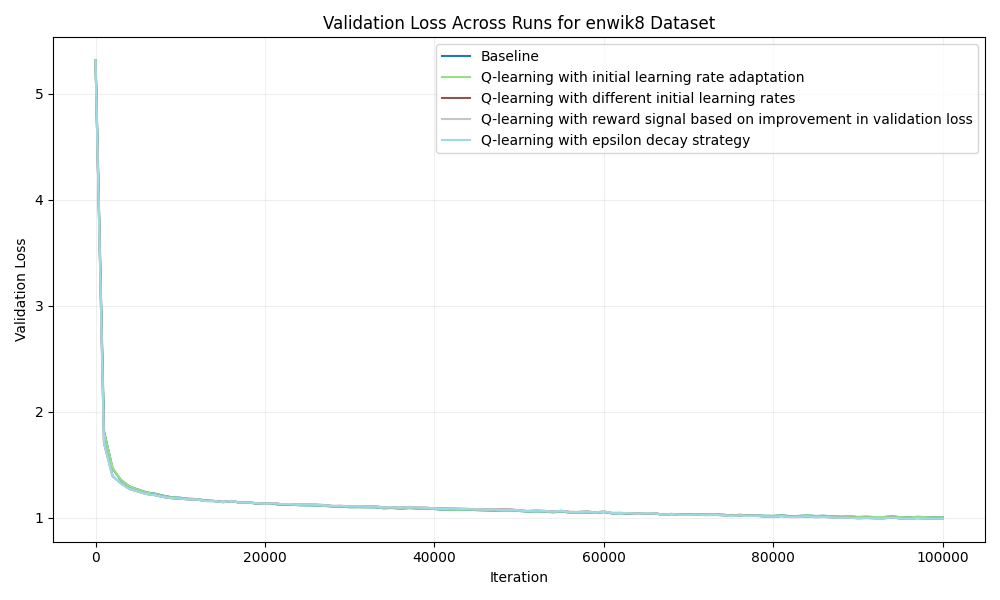
\includegraphics[width=\textwidth]{val_loss_enwik8.png}
        \label{fig:first-run}
    \end{subfigure}
    \hfill
    \begin{subfigure}{0.49\textwidth}
        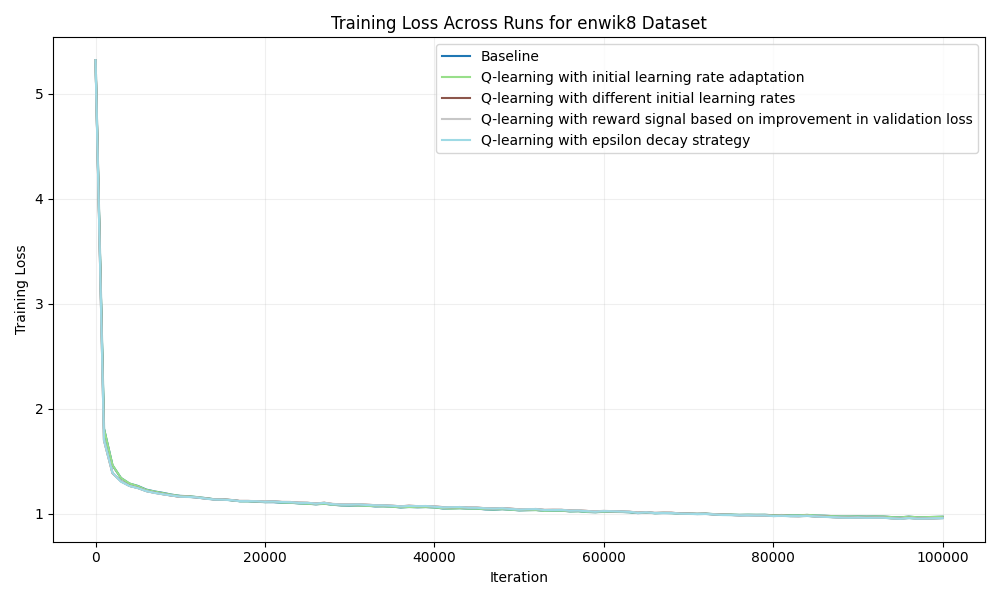
\includegraphics[width=\textwidth]{train_loss_enwik8.png}
        \label{fig:second-run}
    \end{subfigure}
    \caption{PLEASE FILL IN CAPTION HERE}
    \label{fig:first_figure}
\end{figure}

\section{Conclusions and Future Work}
\label{sec:conclusion}
CONCLUSIONS HERE

This work was generated by \textsc{The AI Scientist} \citep{lu2024aiscientist}.

\bibliographystyle{iclr2024_conference}
\bibliography{references}

\end{document}
